\section{Theorie}
\label{sec:Theorie}

Zur Erzeugung von Röntgenstrahlung werden in einer evakuierten Röhre aus einer Glühkathode Elektronen emittiert
und auf eine Anode hin beschleunigt.
Die bei der Kollision austretende Strahlung besteht sowohl aus dem kontinuierlichen Bremsspektrum dargestellt in \autoref{fig:bremsspektrum}, 
als auch aus der charakteristischen Röntgenstrahlung des Anodenmaterials.
\begin{figure}
    \centering
    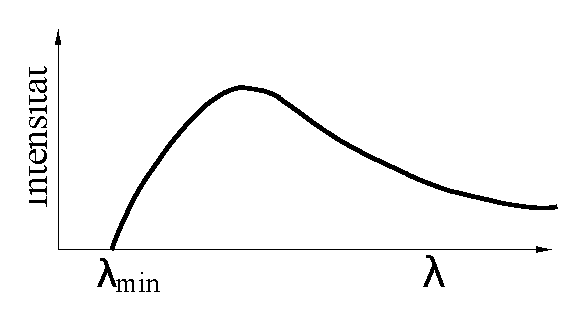
\includegraphics[width=0.6\textwidth]{pictures/bremsspektrum.pdf}
    \caption{Das aufgrund von Energieabgabe kontinuierliche Bremsspektrum des Elektrons. \cite{v602}}
    \label{fig:bremsspektrum}
\end{figure}
Bei der Abbremsung eines Elektrons im Coulombfeld des Atomkerns werden Photonen emittiert, 
deren Energie dem Energieverlust den abgebremsten Elektronen entsprechen.
Die minimale Wellenlänge der Photonen bei vollständiger Abbremsung der Elektronen ergibt sich zu
\begin{equation}
    \lambda_\text{min} = \frac{h \cdot c}{e_0 \, U} \,
\end{equation}
wobei die gesamte kinetische Energie $E_\text{kin} = e_0 \, U$ in Strahlungsenergie umgewandelt wird.

Bei der charakteristischen Röntgenstrahlung wird durch Ionisation des Anodenmaterials ein Elektron in ein energetisch höheres Niveau versetzt,
wodurch ein Röntgenquant mit der Energie $h \, \nu = E_\text{m} - E_\text{n}$ emittiert wird. 
Dies entspricht der Energiedifferenz der beiden Energieniveaus, 
somit besitzt das Röntgenquant eine diskrete Energieverteilung die charakteristisch für das Anodenmaterial der Röntgenröhre.
Diese scharfen Linien werden mit $K_\alpha$, $K_\beta$, $L_\alpha$, ... bezeichnet, wobei $K$, $L$, $M$, ... die Schalen sind, auf denen die Übergänge enden.
Der griechische Buchstabe indiziert, aus welcher Schale das Elektron stammt, welches die innere Schale auffüllt. 

Bei einem Mehrelektronenatom wird die Kernladung durch die Hüllenelektronen und die Wechselwirkung der Elektronen abgeschirmt. 
Aufgrund der Verringerung der Coulomb-Anziehung auf das äußere Elektron ergibt sich für die Bindungsenergie auf der n-ten Schale
\begin{equation}
    E_\text{n} = - E_\text{Ryd} \, z_{\text{eff}}^2 \cdot \frac{1}{n^2} \, .
\end{equation}
Dabei ist $E_\text{Ryd} = \qty{13.6}{eV}$ die Rydbergenergie und $z_\text{eff} = z - \sigma$ die effektive Kernladung mit der Abschirmungskonstante $\sigma$.
Die Abschirmkonstante unterscheidet sich für jedes Elektron und ist empirisch bestimmbar. 
Die Elektronen besitzen neben der Hauptquantenzahl noch weitere Quantenzahlen resultierend aus dem Elektronenspin und dem Bahndrehimpuls, 
sodass eine Feinstruktur ersichtlich wird.
Die Energien dieser Feinstruktur können mithilfe der \textit{Sommerfeldschen Feinstrukturformel}
\begin{equation} \label{eq:feinstruktur}
    E_{\mathrm{n}, \mathrm{j}}= - E_\text{Ryd}\left(z_{\mathrm{eff}}^{2} \, \frac{1}{n^{2}}+\alpha^{2} \, z_{\mathrm{eff}}^{4} \, \frac{1}{n^{3}} \, \left(\frac{1}{j+\frac{1}{2}}-\frac{3}{4 n}\right)\right)
\end{equation}
berechnet werden.
Dabei ist $\alpha$ die Sommerfeldsche Feinstrukturkonstante, $n$ die Hauptquantenzahl und j der Gesamtdrehimpuls des Elektrons.

Bei Absorption von Röntgenstrahlung durch einen Absorber tritt ebenso Charakteristische Röntgenstrahlung auf.
Bei Energien unter 1 MeV treten der Comptoneffekt so wie der Photoeffekt dominant auf. 
Wie in \autoref{fig:absoprtion} dargestellt, nimmt der Absorptionskoeffizient mit zunehmender Energie ab 
und sobald die Photonenenergie die Bindungsenergie eines Elektrons aus der nächsten SChale übersteigt, steigt er schlagartig an.
\begin{figure}[H]
    \centering
    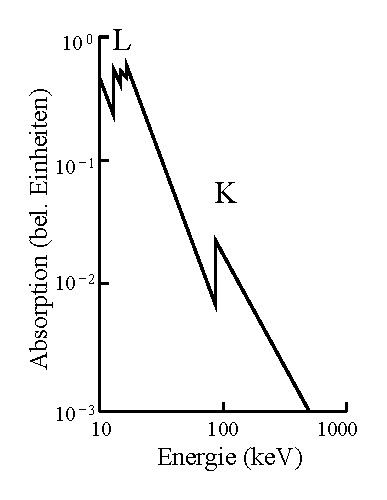
\includegraphics[width=0.4\textwidth]{pictures/absorption.pdf}
    \caption{Das charakteristische Absorptionsspektrum von Röntgenstrahlung. \cite{v602}}
    \label{fig:absoprtion}
\end{figure}
Die Absorptionskanten haben fast die selben Energien wie die Bindungsenergie des Elektrons $h \, \nu_\text{abs} = E_n - E_{\infty}$.
Die zugehörige Energie wird nach der zugehörigen Schale aus denen das Elektron stammt als $K$-, $L$-, $M$-, ... Absorptionskante bezeichnet.
Mithilfe von \autoref{eq:feinstruktur} kann die Abschirmkonstante mit 
\begin{equation} \label{eq:sigma}
    \sigma_{\mathrm{K}}=Z-\sqrt{\frac{E_{\mathrm{K}}}{E_\text{Ryd}}-\frac{\alpha^{2} \, Z^{4}}{4}}
\end{equation}
ermittelt werden.
Der zweite Term unter der Wurzel ber¨ucksichtigt dabei die Feinstrukturaufspaltung der $K$-Schale.
Da die Abschirmzahlen jedel beteiligten Elektrons berücksichtigt werden müssen, 
ergibt sich die Bestimmung der Abschirmkonstante aus der L-Kante unter Berücksichtigung der Feinstruktur als hinreichend kompliziert.
Dies lässt sich jedoch vereinfachen, indem die Energiedifferenzen $\increment E_\text{L}$ zweier Kanten bestimmt werden.
Aufgrund dessen, dass in dem vorliegendem die $L_{I}$- und $L_{II}$-Kante nicht aufgelöst werden können, 
lässt sich die Abschirmkonstante zu 
\begin{equation}
    \sigma_{L}=Z-\left(\frac{4}{\alpha} \sqrt{\frac{\Delta E_{L}}{E_\text{Ryd}}}-\frac{5 \Delta E_{L}}{E_\text{Ryd}}\right)^{1 / 2}\left(1+\frac{19}{32} \alpha^{2} \frac{\Delta E_{L}}{E_\text{Ryd}}\right)^{1 / 2}
\end{equation}
bestimmen. 
Dabei ist die Energiedifferenz $\increment E_\text{L} = E_{L_{II}} - E_{L_{III}}$ und die Ordnungszahl $Z$.

Durch Benutzung der Braggschen Reflexion kann die Energie bzw. die Wellenlänge $\lambda$ der Röntgenstrahlung experimentell analysiert werden. 
Hierbei fällt Röntgenlicht auf ein dreidimensionales Gitter, wobei die Photonen an jedem Atom des Gitters gebeugt werden, wie in \autoref{fig:bragg} dargestellt.
\begin{figure}[H]
    \centering
    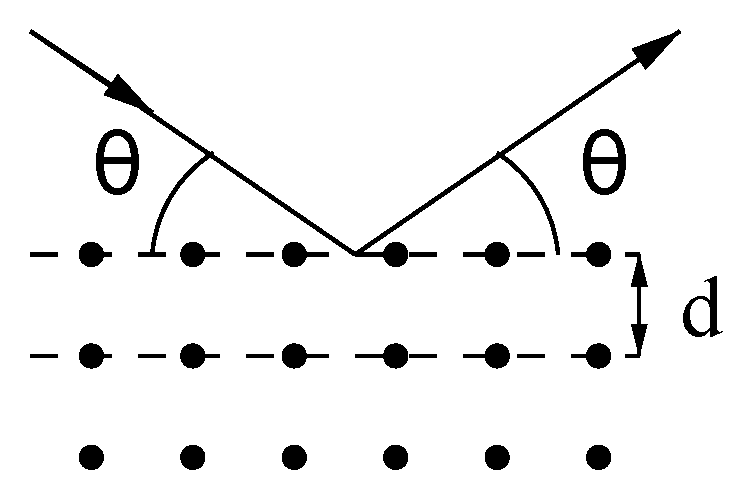
\includegraphics[width=0.4\textwidth]{pictures/bragg.pdf}
    \caption{Die Braggsche Reflexion der Photonen an einem Atomgitter. \cite{v602}}
    \label{fig:bragg}
\end{figure}
Die Strahlen interferieren, während es unter dem Glanzwinkel $\theta$ zu konstruktiverInterferenz kommt. 
So kann mit Hilfe der Braggschen Bedingung
\begin{equation}
    2 \, d \, \sin \theta = n \, \lambda
\end{equation}
und einer bekannten Gitterkonstante $d$ ($d_\text{LIF} = \qty{201.4}{\pico\meter}$ eines LIF-Kristalls) die Wellenlänge bestimmt werden.
Dabei ist $n$ die Beugungsordnung des Maximums.